\documentclass[conference]{IEEEtran}
\IEEEoverridecommandlockouts
\usepackage{cite}
\usepackage{amsmath,amssymb,amsfonts}
\usepackage{graphicx}
\usepackage{textcomp}
\usepackage{xcolor}
\usepackage{booktabs}
\usepackage{array}
\usepackage{multirow}
\usepackage{url}
\usepackage[colorlinks=true,citecolor=blue,linkcolor=blue,urlcolor=blue]{hyperref}
\usepackage{tikz}
\usetikzlibrary{shapes.geometric, arrows.meta, positioning, fit, backgrounds}
\def\BibTeX{{\rm B\kern-.05em{\sc i\kern-.025em b}\kern-.08em
    T\kern-.1667em\lower.7ex\hbox{E}\kern-.125emX}}
\begin{document}
\pagestyle{plain}
\pagenumbering{arabic}
\title{An Explainable ML Risk Alarm Layer to Assist Deterministic Policy Decisions in Zero Trust Architecture for IIoT Security}

\author{
\IEEEauthorblockN{Prerak Patel}
\IEEEauthorblockA{\textit{Computer Engineering} \\
\textit{Florida Institute of Technology}\\
}
}

\maketitle
\thispagestyle{plain}

\begin{abstract}
Zero Trust Architecture (ZTA) relies on a Policy Engine that verifies every access request against identity, device posture, and context. The model is a good fit for Industrial Internet of Things (IIoT) environments where safety and compliance are non-negotiable, but deploying ZTA at the network edge introduces real problems in identity management, secrets distribution, and policy enforcement that centralized designs sidestep rather than solve. Recent work has brought machine learning into ZTA for intrusion detection and trust scoring, but those efforts either hand ML autonomous authorization authority or treat explainability as someone else's problem. This paper proposes a two-stage decision framework: deterministic policy enforcement retains sole authorization authority, and a lightweight ML risk alarm layer flags anomalous requests that already cleared policy. The ML layer evaluates contextual signals (device attestation, geolocation deviation, time-of-access patterns, behavioral baseline divergence, request velocity) using gradient-boosted tree classifiers. SHAP provides per-prediction feature attribution, and DiCE generates counterfactual explanations for offline policy debugging. A concrete edge deployment stack is specified using K3s, SPIRE, HashiCorp Vault, and Keycloak, each mapped to a ZTA logical component. Because representative IIoT access logs are scarce and often proprietary, the dataset challenge is documented and an LLM-based synthetic data generation approach is described as an academic bootstrap exercise. A proof-of-concept evaluation on synthetic data is included; empirical validation on real logs remains future work.
\end{abstract}

\begin{IEEEkeywords}
Zero Trust Architecture, Explainable AI, Industrial IoT, SHAP, Counterfactual Explanations, Anomaly Detection, Policy Engine, Edge Computing, Kubernetes, SPIRE, Vault, Keycloak, Synthetic Data
\end{IEEEkeywords}

%===================================================================
\section{Introduction}
%===================================================================

Zero Trust Architecture (ZTA) treats every access request as potentially hostile and verifies each one against identity, device posture, and context~\cite{kindervag2010, nist800207}. The model is a reasonable fit for Industrial Internet of Things (IIoT) environments, where safety-critical infrastructure, legacy protocols, and geographic distribution make perimeter-based security untenable~\cite{zanasi2024, ehrlich2021}. NIST SP 800-207 already anticipates dynamic, risk-informed decisions through its Trust Algorithm, which can flag contextual anomalies like a bulk export from an unfamiliar location at 3~AM~\cite{nist800207}. That is where ML is useful.

The problem is how ML gets used. Fewer than 30\% of IoT-focused ZTA implementations include any environmental perception module~\cite{azad2024}, and where ML does appear it typically acts as the decision-maker rather than an advisory layer~\cite{laghari2025}. Handing authorization authority to an opaque model creates an audit gap that matters in safety-critical plants: an incorrect denial can have physical consequences, and ``the model scored this below threshold'' does not satisfy a safety regulator or an incident postmortem~\cite{capuano2022}. Explainability is conspicuously absent too: Ramezanpour and Jagannath~\cite{ramezanpour2022} introduced the Monitor-Evaluate-Decide paradigm for ML-enabled ZTA but left transparency unaddressed. No existing work, to our knowledge, places an explainable ML advisory layer explicitly alongside (not inside) a deterministic ZTA enforcement path for IIoT.

This paper proposes a two-stage design that separates enforcement from risk awareness. A deterministic policy gate is the sole authority on granting or denying access. For requests that clear that gate, a secondary ML classifier evaluates contextual signals and flags anomalies. The classifier has no enforcement path; it produces alerts, risk scores, and audit records.

For the ML layer's risk assessments to be useful to analysts, they need to be inspectable. The framework uses SHAP (SHapley Additive exPlanations)~\cite{lundberg2017} for feature-level attribution (e.g., ``this request was flagged primarily because of the 3~AM access time and the 400~km geolocation deviation'') and DiCE (Diverse Counterfactual Explanations)~\cite{mothilal2020} for offline policy debugging. Both operate asynchronously outside the enforcement path. Neither eliminates the known stability limitations of post-hoc explanation methods near decision boundaries~\cite{alvarez2018, jiang2024}; the framework addresses this through explicit stability evaluation rather than assuming reliable explanations in all cases. Rastogi et al.~\cite{rastogi2025} found that nearly two-thirds of SOC analysts distrust AI alerts lacking clear explanations, and that feature contribution breakdowns are the most requested explanation form. That is precisely what SHAP produces.

The contributions of this paper are as follows:
\begin{enumerate}
    \item A synthesis of literature across ZTA, IIoT security, ML-based anomaly detection, and XAI, identifying a gap at their intersection that has not been addressed.
    \item A two-stage architecture in which deterministic ZTA policy retains authority while an explainable ML layer adds risk awareness.
    \item A concrete edge deployment stack mapping open-source tools (K3s, SPIRE, Vault, Keycloak) to ZTA components, grounded in their respective specifications.
    \item A description of how SHAP and DiCE fill complementary roles: analyst trust, audit trails, and policy debugging.
    \item An honest account of the dataset problem for IIoT access anomaly detection and an LLM-based synthetic data generation approach as an academic bootstrap exercise.
    \item A transparent framing of this work as a conceptual framework with stated limitations and evaluation plans.
\end{enumerate}

The framework is designed to investigate three research questions:
\begin{itemize}
    \item[\textbf{RQ1.}] Can a secondary ML alarm layer detect contextual anomalies in policy-authorized IIoT access requests without degrading the deterministic enforcement path?
    \item[\textbf{RQ2.}] Do SHAP feature attributions and DiCE counterfactual explanations produce stable, actionable outputs for SOC analysts reviewing flagged access events?
    \item[\textbf{RQ3.}] Does the two-stage design reduce the operational risk of ML false positives and false negatives compared to architectures where ML directly controls authorization?
\end{itemize}

%===================================================================
\section{Related Work}
%===================================================================

\subsection{Zero Trust Architecture Foundations}

Kindervag at Forrester Research coined the term ``zero trust'' in 2010, arguing that perimeter-based security fails because it treats internal traffic as trustworthy by default~\cite{kindervag2010}. NIST SP 800-207 formalized the idea with a reference architecture centered on the Policy Decision Point (PDP), which consists of the Policy Engine and Policy Administrator and instructs the PEP to allow or block communication~\cite{nist800207}. The document lays out seven tenets, three deployment approaches (enhanced identity governance, micro-segmentation, software-defined perimeters), and a Trust Algorithm that can use criteria-based or score-based evaluation. Notably, NIST states that the weighting may be ``a proprietary algorithm''~\cite{nist800207}, an implicit acknowledgment that scoring mechanisms may lack transparency.

Several surveys have since mapped the field. Syed et al.~\cite{syed2022} produced one of the most cited ZTA reviews, covering identity management, micro-segmentation, and security analytics while pointing out that trust assessment and continuous monitoring lag behind authentication research. He et al.~\cite{he2022} cataloged practical challenges: policy management complexity, scalability limitations, and the tension between security and usability. Liu et al.~\cite{liuzt2024} ran a bibliometric analysis and found that AI/ML convergence with ZTA is an emerging but still sparse research area. On the institutional side, the Department of Defense Zero Trust Reference Architecture added a dedicated visibility and analytics pillar for behavioral monitoring~\cite{dodzta2022}. NIST SP 1800-35~\cite{nist180035} then demonstrated 19 real implementations with continuous risk-based assessment, moving the field from abstract reference architecture toward operational deployment.

\subsection{Zero Trust in IIoT and Cyber-Physical Systems}

IIoT environments bring problems that conventional enterprise IT does not have. Zanasi et al.~\cite{zanasi2024} built a flexible ZTA for IIoT using SDN-based micro-segmentation and showed that identity-centric zero trust can work in industrial settings, though they did not address dynamic risk assessment. Feng and Hu~\cite{feng2023} developed a Cyber-Physical ZTA with a multi-layer access control engine that evaluates trust scores across the boundary between cyber and physical domains. Pliatsios et al.~\cite{pliatsios2023} implemented a ZTA for IIoT remote access with multi-level authorization using open-source tools, but included no anomaly detection or ML.

The legacy device problem is particularly stubborn. Ehrlich et al.~\cite{ehrlich2021} derived 12 rules for integrating sensors, actuators, and controllers that run insecure protocols (Modbus, DNP3) and lack encryption. Azad et al.~\cite{azad2024} found in a multidimensional survey that fewer than 30\% of IoT ZTA papers implement environmental perception modules, even though contextual awareness is central to the Zero Trust idea. Wang et al.~\cite{wangzt2025} concluded in a 2025 review that ZT research in IIoT is still in early stages, especially regarding trust evaluation.

A common pattern runs through these works: when ML appears, it operates as the primary decision-maker inside detection or authentication pipelines, not as a separate, interpretable advisory layer alongside deterministic policy.

\subsection{ML for Risk Scoring and Anomaly Detection}

ML-based anomaly detection has a long track record in cybersecurity. Chandola et al.~\cite{chandola2009} established a taxonomy distinguishing point, contextual, and collective anomalies, all of which apply to access request analysis. Ali et al.~\cite{ali2024} surveyed ML algorithms for intrusion detection and reported that Random Forests reach 95.2\% accuracy with 15.7ms processing time, which shows that lightweight models can handle real-time risk scoring. Mahansaria and Roy~\cite{mahansaria2024} found that adding contextual signals (device attributes, user behavior, network context) to ML authentication models improves detection of DoS and brute-force attacks compared to context-free baselines.

On the architectural side, Ramezanpour and Jagannath~\cite{ramezanpour2022} introduced the intelligent ZTA (i-ZTA) framework with a Monitor-Evaluate-Decide paradigm, the first formal blueprint for ML-integrated Zero Trust policy engines. Laghari et al.~\cite{laghari2025} reached 99.82\% accuracy with XGBoost for intrusion detection within ZTA for IIoT. Jeong and Yang~\cite{jeong2025} decomposed trust into user behavior, network environment, device status, and threat history, with sensitivity analysis indicating that behavior and network context matter most. None of these works, however, address the explainability of their ML components, and most treat ML as the authoritative decision-maker rather than a secondary layer.

\subsection{Explainable AI in Cybersecurity}

Capuano et al.~\cite{capuano2022} produced the first broad IEEE survey of XAI in cybersecurity, covering intrusion detection, malware analysis, phishing, and digital forensics. They split techniques into ante-hoc (inherently interpretable) and post-hoc (explanation after prediction) categories and found that post-hoc methods dominate because complex models tend to be more accurate. Mohale and Obagbuwa~\cite{mohale2025} reviewed XAI integration in intrusion detection specifically and found that SHAP provides consistent global and local feature attributions without excessive computational cost.

On the practitioner side, Rastogi et al.~\cite{rastogi2025} surveyed SOC analysts and found that nearly two-thirds distrust AI alerts that lack clear explanations. Feature contribution explanations and confidence scores were the most requested types, which maps well onto what SHAP produces. Yan et al.~\cite{yan2022} reported that interactive dashboards with XAI reduce incident resolution time by about 30\%. The message from this literature is consistent: explainability is an operational requirement for deployed security models, not an optional academic exercise.

\subsection{SHAP, Counterfactual Methods, and Explanation Robustness}

Lundberg and Lee~\cite{lundberg2017} introduced SHAP, which assigns each feature an importance value for a given prediction based on Shapley values from cooperative game theory. The method guarantees local accuracy, missingness, and consistency. TreeSHAP computes exact Shapley values in polynomial time for tree-based models. Alenezi and Ludwig~\cite{alenezi2021} applied TreeSHAP, KernelSHAP, and DeepSHAP to Random Forest and XGBoost classifiers on cybersecurity datasets and confirmed that SHAP produces interpretable feature attributions across different threat types.

Mothilal et al.~\cite{mothilal2020} proposed DiCE, which generates diverse counterfactual explanations through constrained optimization. It identifies minimal, feasible input changes that would flip a prediction. In a behavioral study, Schemmer et al.~\cite{schemmer2023} found that counterfactual explanations improve both the accuracy and speed of human anomaly investigation, giving empirical support to the idea that counterfactuals help analysts reason about decision boundaries. Verma et al.~\cite{verma2024} cataloged over 350 counterfactual methods and established evaluation criteria (validity, proximity, sparsity, diversity, actionability) that apply to security use cases.

There are known risks. Alvarez-Melis and Jaakkola~\cite{alvarez2018} showed that post-hoc explanations can be unstable when inputs change slightly. Jiang et al.~\cite{jiang2024} surveyed robust counterfactual explanations and found that many methods produce explanations that break after model retraining, which matters for any deployed security system. Galinkin~\cite{galinkin2022}, writing from the cybersecurity firm Rapid7, assessed SHAP from a practitioner perspective and warned that explanation instability is not just a theoretical concern but a practical one, motivating stability testing before deployment.

\subsection{Research Gap}

The threads reviewed above do not connect. Papers combining ZTA with ML for IIoT~\cite{laghari2025, feng2023} treat the ML model as the decision authority and omit any explainability. Papers combining ZTA with XAI~\cite{haque2024, nkoro2024} work in narrow domains (UAV networks, generic enterprise IT) without the operational and legacy-device constraints that define IIoT. Context-aware ZTA trust scoring papers~\cite{xiao2022, jeong2025} formalize the right signals but either stop short of ML or skip explainability. Marquez~\cite{marquez2025} sketched an explainable zero-trust identity framework for industrial environments and then offered nothing in the way of model selection, implementation, or evaluation. To our knowledge, no existing work positions an explainable ML risk classifier as an advisory layer explicitly subordinate to deterministic policy, with the IIoT operational context taken seriously throughout. That is the gap this paper addresses.

%===================================================================
\section{Proposed Framework}
%===================================================================

\subsection{Threat Model and System Assumptions}

The adversary model assumes an attacker who has obtained valid credentials (through phishing, credential stuffing, or insider compromise) and can pass deterministic policy checks. The attacker's goal is to access IIoT resources (sensor data, control commands, configuration endpoints) while appearing authorized. We assume the adversary cannot compromise the PE/PA/PEP infrastructure itself, the SIEM pipeline, or the telemetry collection agents; these are trusted components. The assets under protection are IIoT operational resources: SCADA interfaces, historian databases, PLC programming endpoints, and sensor telemetry streams.

The ML alarm layer targets a specific blind spot: access that is \textit{authorized but contextually anomalous}. A legitimate operator credential used from an unfamiliar location at 3~AM to pull bulk historian data would pass deterministic policy but should raise an alarm. We assume that telemetry signals (device posture, geolocation, timing, behavioral history) are collected faithfully and not spoofed at the collection point. If an attacker can manipulate telemetry before it reaches the ML layer, the alarm layer can be evaded, a limitation shared with any monitoring system that trusts its own instrumentation.

\subsection{Design Philosophy}

The core constraint is simple: nothing in this design lets the ML model grant or deny access. That boundary is non-negotiable. In IIoT and safety-critical environments, allowing an opaque model to block a process engineer's request to a PLC, or to permit one that a rule would have blocked, is not a calculated risk tradeoff. It is an organizational and regulatory failure waiting to happen. Deterministic rules can be audited, argued about, and updated through a governance process. A gradient-boosted tree's reasoning cannot be argued about in a control room at 2~AM. The two things are not substitutable~\cite{nist800207, ehrlich2021}.

Given that constraint, the ML layer's role is strictly advisory: evaluate contextual characteristics, produce a risk score, log it, raise an alert if warranted. It has no path to enforcement. The system's safety properties are determined entirely by the deterministic policy; the ML component can only add visibility on top, never subtract it.

\subsection{Learning Formulation}

The ML layer operates as a supervised binary classifier trained on labeled access logs, where each record is labeled as \textit{normal} or \textit{anomalous} based on historical incident data and analyst annotations. The input is a feature vector $\mathbf{x} \in \mathbb{R}^d$ constructed from the contextual signals described in Section~III-E. The model outputs a risk score $s(\mathbf{x}) \in [0, 1]$, and a configurable threshold $\tau$ determines whether the request is flagged: $\text{flag}(\mathbf{x}) = \mathbf{1}[s(\mathbf{x}) > \tau]$. Because false positives generate alerts rather than access denials, $\tau$ can be tuned toward higher recall without the operational penalty that would exist in a blocking architecture.

\textbf{Class imbalance.} Anomalous access events are rare. In practice, class ratios of 100:1 or worse are realistic for IIoT access logs, so standard cross-entropy training learns to predict the majority class almost exclusively. The training procedure must apply class-weighted loss or SMOTE-style oversampling~\cite{ali2024}. Evaluation should report F1 and AUC-ROC rather than accuracy: a classifier that never fires can hit 99\% accuracy on a skewed dataset and be operationally worthless. Several papers cited in this review report accuracy figures on intrusion detection benchmarks without disclosing class distributions, which makes those numbers difficult to interpret.

\textbf{Score calibration.} The raw output $s(\mathbf{x})$ from a gradient-boosted classifier is not a calibrated probability. Without Platt scaling or isotonic regression on a held-out set, a score of 0.82 means only ``higher than 0.6,'' not ``82\% likely anomalous.'' Calibration is required before scores carry interpretable meaning for analysts, especially when attached to SHAP attributions. Threshold $\tau$ should be derived from precision-recall curves on held-out data after calibration, not picked by hand.

\textbf{Concept drift.} IIoT access patterns shift as deployments evolve: new devices come online, shift schedules change, staff rotate. A model trained on last year's logs can degrade silently, and in a monitoring-without-blocking design that means missed alarms accumulate without any visible failure. The framework includes drift monitoring via population stability index on feature distributions, with retraining triggered when shift exceeds a deployment-defined threshold. This creates a secondary problem: Jiang et al.~\cite{jiang2024} showed counterfactual explanations become invalid after model updates. A version-controlled explanation store is therefore needed so historical alerts are not retroactively re-explained by a model the analyst never saw.

\textbf{Analyst feedback loops.} Analyst verdicts on flagged alerts (escalated, dismissed, confirmed true positive) are the highest-quality labeling signal available for improving the model. The framework includes a structured feedback interface that writes analyst dispositions back to the training corpus. The dependency is real and constraining: the model only improves as fast as analysts label, and in understaffed SOC environments that feedback arrives slowly. Threshold recalibration between full retraining cycles absorbs some of this lag, but deployment planning should account for it rather than assuming labels arrive on schedule.

In deployments where labeled anomaly data is scarce initially, the classifier can be bootstrapped using semi-supervised learning: training on verified-normal access patterns and treating statistical outliers as candidate anomalies for analyst review. Once analysts label a sufficient corpus of flagged events, the model transitions to fully supervised training on a rolling window of recent logs.

\subsection{Two-Stage Decision Architecture}

The framework implements a two-stage process aligned with NIST SP 800-207 and the MED paradigm~\cite{ramezanpour2022}.

\textbf{Stage 1: Deterministic Policy Evaluation.} When an access request arrives at the PEP, the PE applies deterministic policies: identity and authentication credentials, role-based or attribute-based permissions, device compliance status (via CDM), and resource-specific access rules. If any criterion fails, the request is denied. This denial is final; the ML layer is not consulted for denied requests.

\textbf{Stage 2: ML Risk Alarm Evaluation.} For requests satisfying all deterministic criteria, the ML layer performs contextual evaluation. It produces a risk score and, when the score exceeds a configured threshold, generates a risk flag. Possible responses include:
\begin{itemize}
    \item \textbf{Logging:} Risk flag, score, and feature contributions recorded in SIEM.
    \item \textbf{Analyst alerting:} Notification to SOC for review, with SHAP-based explanation attached.
    \item \textbf{Enhanced monitoring:} Session marked for elevated scrutiny.
    \item \textbf{Optional step-up challenge:} Additional authentication may be requested (deployment-dependent).
\end{itemize}

Even when a risk flag is raised, access proceeds because the deterministic policy has already authorized it. The risk flag creates an audit record and triggers monitoring responses but does not override the policy decision.

Fig.~\ref{fig:architecture} illustrates the proposed architecture.

\begin{figure}[!ht]
\centering
\resizebox{0.95\columnwidth}{!}{%
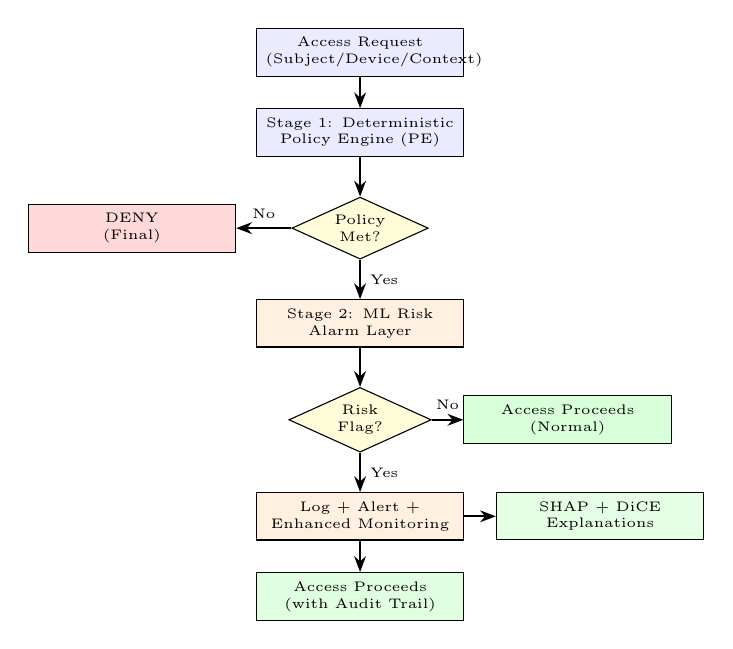
\begin{tikzpicture}[
    node distance=0.4cm and 0.25cm,
    block/.style={rectangle, draw, fill=blue!8, text width=2.4cm, minimum height=0.6cm, align=center, font=\tiny},
    mlblock/.style={rectangle, draw, fill=orange!12, text width=2.4cm, minimum height=0.6cm, align=center, font=\tiny},
    xaiblock/.style={rectangle, draw, fill=green!10, text width=2.4cm, minimum height=0.6cm, align=center, font=\tiny},
    decision/.style={diamond, draw, fill=yellow!15, aspect=2.2, inner sep=0pt, font=\tiny, text width=1cm, align=center},
    arrow/.style={-Stealth, semithick},
    every node/.style={font=\tiny}
]

% Nodes
\node[block] (req) {Access Request\\(Subject/Device/Context)};
\node[block, below=0.4cm of req] (pe) {Stage 1: Deterministic\\Policy Engine (PE)};
\node[decision, below=0.5cm of pe] (dec1) {Policy\\Met?};
\node[block, left=0.7cm of dec1, fill=red!15] (deny) {DENY\\(Final)};
\node[mlblock, below=0.5cm of dec1] (ml) {Stage 2: ML Risk\\Alarm Layer};
\node[decision, below=0.5cm of ml] (dec2) {Risk\\Flag?};
\node[block, right=0.4cm of dec2, fill=green!15] (normal) {Access Proceeds\\(Normal)};
\node[mlblock, below=0.5cm of dec2] (alert) {Log + Alert +\\Enhanced Monitoring};
\node[block, below=0.4cm of alert, fill=green!12] (proceed) {Access Proceeds\\(with Audit Trail)};
\node[xaiblock, right=0.4cm of alert] (xai) {SHAP + DiCE\\Explanations};

% Arrows
\draw[arrow] (req) -- (pe);
\draw[arrow] (pe) -- (dec1);
\draw[arrow] (dec1) -- node[above] {No} (deny);
\draw[arrow] (dec1) -- node[right] {Yes} (ml);
\draw[arrow] (ml) -- (dec2);
\draw[arrow] (dec2) -- node[above] {No} (normal);
\draw[arrow] (dec2) -- node[right] {Yes} (alert);
\draw[arrow] (alert) -- (proceed);
\draw[arrow] (alert) -- (xai);

\end{tikzpicture}%
}
\caption{Proposed two-stage Zero Trust decision architecture. The deterministic policy gate (Stage~1) retains sole authorization authority. The ML alarm layer (Stage~2) evaluates contextual anomalies for authorized requests. SHAP and DiCE provide offline analyst-facing explainability.}
\label{fig:architecture}
\end{figure}

\subsection{Feature Set and Signal Categories}

The ML layer evaluates contextual signals aligned with the NIST SP 800-207 Trust Algorithm inputs and validated by recent contextual authentication research~\cite{mahansaria2024, xiao2022}. Following the trust score decomposition of Jeong and Yang~\cite{jeong2025}, features are organized into four categories:

\textbf{User features.} Behavioral baseline divergence: deviations in access patterns, resource usage, or interaction sequences relative to historical profiles. Request velocity and burstiness: unusual spikes in access request rates or anomalous clustering. Time-of-access deviation: requests outside expected operational hours. These signals apply to both human operators and service accounts.

\textbf{Device features.} Device posture and attestation: OS version, patch level, firmware integrity, and hardware attestation status against compliance baselines. For IIoT, many legacy devices (PLCs, RTUs) lack attestation capabilities entirely~\cite{ehrlich2021}; the feature vector encodes attestation-absent as a distinct category rather than treating it as a failure signal.

\textbf{Session features.} Protocol type, payload size, command sequences, and session duration relative to historical profiles. In IIoT, command sequences are often highly regular (e.g., periodic sensor polls), making deviations more informative than in enterprise environments.

\textbf{Environment features.} Geolocation anomaly: deviation from the subject's established location baseline, including impossible travel detection. This signal is most informative for mobile operators and remote access; for fixed industrial devices with static IP assignments, geolocation carries less weight and the model should reflect that through lower feature importance.

Jeong and Yang's sensitivity analysis~\cite{jeong2025} indicates that user behavior and network context are the most influential factors in real-time trust scoring, which aligns with our feature prioritization.

\subsection{ML Model Considerations}

The ML layer should use lightweight models suited to tabular access log data. Ali et al.~\cite{ali2024} benchmarked Random Forests at 95.2\% accuracy with 15.7ms processing time on intrusion detection tasks. Laghari et al.~\cite{laghari2025} reached 99.82\% accuracy with XGBoost in IIoT environments. Gradient-boosted trees (XGBoost, LightGBM) are a good fit: they are computationally efficient, compatible with TreeSHAP for fast explanation generation~\cite{lundberg2017}, and designed for exactly the kind of structured tabular data that access logs produce. Deep learning would add latency and explanation complexity for a secondary alarm layer that operates on engineered features, without clear accuracy gains on tabular inputs.

\subsection{Explainability Components}

\textbf{SHAP for feature-level attribution.} When a risk flag is generated, SHAP values indicate each feature's contribution to the risk score. TreeSHAP computes exact Shapley values in polynomial time for tree-based models~\cite{lundberg2017}. Alenezi and Ludwig~\cite{alenezi2021} demonstrated that SHAP provides meaningful, interpretable feature attributions across cybersecurity domains. Mohale and Obagbuwa~\cite{mohale2025} confirmed that SHAP excels in consistency and computational feasibility for IDS applications.

\textbf{DiCE for counterfactual analysis.} DiCE generates diverse counterfactual explanations identifying minimal feasible changes that would alter the risk classification~\cite{mothilal2020}. Schemmer et al.~\cite{schemmer2023} provided empirical evidence that counterfactual explanations significantly improve human accuracy in anomaly investigation. Use cases include policy debugging (``what conditions would make this request non-risky?''), post-incident analysis, and policy refinement.

Table~\ref{tab:shap_dice} summarizes the complementary roles of SHAP and DiCE.

\begin{table}[t]
\centering
\caption{Complementary roles of SHAP and DiCE in the proposed framework.}
\label{tab:shap_dice}
\begin{tabular}{p{1.8cm}p{2.8cm}p{2.8cm}}
\toprule
\textbf{Aspect} & \textbf{SHAP} & \textbf{DiCE} \\
\midrule
Question & ``Why was this flagged?'' & ``What would change the flag?'' \\
\addlinespace
Output & Feature importance values per prediction & Alternative scenarios that flip prediction \\
\addlinespace
Use case & Alert triage, audit logging, compliance & Policy debugging, root cause analysis \\
\addlinespace
Timing & Near-real-time (TreeSHAP) & Primarily offline, on-demand \\
\addlinespace
Basis & Shapley values (game theory) & Constrained optimization with diversity \\
\addlinespace
Evaluation & Local accuracy, consistency~\cite{lundberg2017} & Validity, proximity, sparsity~\cite{verma2024} \\
\bottomrule
\end{tabular}
\end{table}

\subsection{Integration with ZTA Components}

The ML layer receives contextual data from the same sources that feed the PE's Trust Algorithm: CDM systems, activity logs, threat intelligence, and SIEM. Risk scores and SHAP attributions are published to the SIEM system, creating a unified audit trail alongside deterministic access decisions. DiCE reports are generated on demand for analyst investigation. The Explanation Module operates asynchronously, introducing no additional latency into the enforcement path. This positioning aligns with the finding by Rastogi et al.~\cite{rastogi2025} that SOC analysts prefer feature contribution explanations attached to alerts rather than requiring separate investigation tools.

\subsection{Worked Example}

Consider a concrete scenario. An operator with valid credentials and an authorized role requests read access to a SCADA historian database at 2:47~AM from a VPN endpoint geolocated 400~km from the plant. The deterministic policy gate checks identity, role permissions, device compliance, and resource access rules; all pass. The request is authorized.

The ML layer then evaluates contextual signals for this authorized request. The feature vector shows: time-of-access deviation is high (the operator's historical access window is 7~AM--6~PM), geolocation distance from baseline is 400~km, request targets a bulk data export endpoint rarely used by this role, and request velocity is normal. The gradient-boosted classifier produces a risk score of 0.82, exceeding the configured threshold $\tau = 0.6$. A risk flag is generated.

SHAP attribution for this prediction shows: time-of-access deviation contributes +0.31 to the risk score, geolocation anomaly contributes +0.24, and target resource rarity contributes +0.19. The remaining features contribute smaller amounts. The analyst sees immediately that timing and location drove the flag, not velocity or device posture.

On-demand, the analyst requests a DiCE counterfactual: ``What would make this request non-risky?'' DiCE returns: if the same request occurred between 7~AM and 6~PM \textit{and} from within 50~km of the plant, the risk score would drop to 0.23. This tells the analyst the flag is not about the data access itself but about when and where it happened, which is useful context for deciding whether to escalate or close the alert.

Access was never blocked. The operator got in. But the SOC has a structured record of why the ML layer flagged this session, and the analyst can make an informed judgment.

%===================================================================
\section{Edge Systems Architecture}
%===================================================================

The two-stage ZTA framework described in Section~III is a logical design. Making it operational in an IIoT edge environment requires mapping each logical component to a concrete technology that can run on resource-constrained infrastructure, tolerate intermittent connectivity to a central control plane, and satisfy the identity and secrets management requirements that Zero Trust demands. This section describes a proposed open-source deployment stack and explains how each tool serves the ZTA architecture.

\subsection{Deployment Context: Why the Edge Matters}

IIoT deployments are not centralized. Sensors, PLCs, and SCADA gateways operate at physical sites that may be geographically remote, connected to enterprise networks over limited or unreliable WAN links, and staffed infrequently. A ZTA design that requires a round-trip to a central Policy Engine for every access decision introduces unacceptable latency for time-sensitive control systems and becomes a single point of failure for the entire site when connectivity drops. The edge architecture proposed here places the Policy Enforcement Point (PEP) and a local instance of the Policy Engine (PE) on-site, synchronized with a central control plane during normal operation and able to apply cached policy decisions during brief connectivity gaps.

This edge-local design is consistent with NIST SP 800-207's acknowledgment that policy decision components may be distributed~\cite{nist800207} and with the micro-segmentation approach documented in NIST SP 1800-35~\cite{nist180035}. It also addresses the operational reality documented by Ehrlich et al.~\cite{ehrlich2021}: legacy OT devices on the shop floor cannot be moved closer to a cloud PDP, so the PDP must be moved closer to them.

\subsection{Container Orchestration: Docker and K3s}

All ZTA components in the proposed stack run as containers managed by K3s, a CNCF-certified lightweight Kubernetes distribution designed for resource-constrained and edge environments~\cite{k3s2024}. K3s packages the Kubernetes control plane into a single binary under 100~MB, supports ARM and x86 architectures, and is designed for nodes with as little as 512~MB of RAM, making it deployable on industrial edge hardware such as ruggedized servers or edge gateways that sit alongside OT equipment.

Docker provides the container runtime layer. Each ZTA logical component runs in its own container: the PEP as an Envoy proxy sidecar or standalone gateway, the local PE as a policy evaluation service (e.g., Open Policy Agent), the ML risk alarm service, and the SIEM log forwarder. K3s manages scheduling, health monitoring, restart policies, and rolling updates for all of these, applying exactly the same operational model that enterprise Kubernetes clusters use but at edge scale.

The value for ZTA is isolation and consistency. Container boundaries enforce the separation of concerns that the two-stage design requires: the deterministic PE container has no network path to the ML container's enforcement interface, making the advisory-only constraint structural rather than just policy. K3s Network Policies implement micro-segmentation at the pod level, restricting which components can communicate and over which ports, aligned with the software-defined perimeter approach described in NIST SP 800-207~\cite{nist800207}.

\subsection{Workload Identity: SPIRE and SPIFFE}

A Zero Trust architecture cannot rely on network location as a trust signal. Each workload (container, service, edge device agent) needs a cryptographically verifiable identity that is independent of its IP address. The SPIFFE (Secure Production Identity Framework for Everyone) standard and its reference implementation, SPIRE (SPIFFE Runtime Environment), provide exactly this~\cite{spiffe2023}.

SPIRE operates as a server-agent architecture. A SPIRE Server runs at the central control plane (or is federated across sites). A SPIRE Agent runs on each K3s node. When a workload starts, the SPIRE Agent attests it using node-level attestation (TPM, cloud instance metadata, or Kubernetes service account tokens) and workload-level attestation (container image hash, pod labels, process metadata). On successful attestation, the agent delivers an SVID (SPIFFE Verifiable Identity Document) to the workload: an X.509 certificate or JWT whose Subject Alternative Name encodes a SPIFFE ID in URI form (e.g., \texttt{spiffe://zt-iiot.local/pe/policy-engine}).

In the proposed ZTA stack, every component that participates in access control carries an SVID. The PE presents its SVID to the PEP when pushing policy updates. The ML service presents its SVID when writing risk scores to the SIEM. The PEP validates the SVID of any component attempting to connect before accepting its input. This establishes mutual TLS (mTLS) between all ZTA services without requiring static certificates or pre-shared keys, replacing network-perimeter trust with identity-based trust throughout the enforcement path.

SPIRE's short-lived certificate rotation (configurable from minutes to hours) limits the blast radius of a compromised credential. If an attacker obtains an SVID, it expires quickly and cannot be renewed without re-passing attestation. This property is particularly important in IIoT environments where devices may be physically accessible to attackers.

\subsection{Secrets and PKI Management: HashiCorp Vault}

ZTA components require secrets: TLS private keys, API credentials for SIEM integration, database passwords for policy stores, and ML model signing keys. Hardcoded secrets in container images or environment variables are a persistent source of credential exposure in containerized deployments. HashiCorp Vault provides a centralized secrets management service with dynamic secret generation, fine-grained access control, and full audit logging~\cite{vault2024}.

In the proposed stack, Vault serves two primary roles. First, it acts as the intermediate Certificate Authority for the ZTA deployment, issuing TLS certificates to components that do not use SPIFFE (e.g., legacy OT gateway integrations). The Vault PKI secrets engine can sign certificates for specific domains and enforce short TTLs with automatic rotation, reducing the window of exposure for any compromised certificate. Second, it issues dynamic credentials for short-lived access: rather than storing a static database password, the PE requests a credential from Vault at startup, receives a time-limited credential generated specifically for that instance, and the credential is revoked when the instance stops.

Vault authentication for ZTA workloads is handled through the Kubernetes auth method, which validates the Kubernetes service account token of a pod before issuing secrets. Combined with SPIRE-issued SVIDs, this creates two independent attestation paths for workload identity: Vault trusts Kubernetes, and SPIRE trusts the workload's runtime attestation. The combination means a compromised container image alone is not sufficient to obtain secrets, because the attacker would also need a valid Kubernetes service account token bound to the correct namespace and service account.

Vault's audit log records every secret access with timestamp, identity, and the specific secret path requested. In a ZTA context, this produces a complete trail of which component accessed which credential and when, complementing the access log produced by the PEP and the risk score log produced by the ML layer.

\subsection{Identity Provider and Federation: Keycloak}

Human operators and service accounts authenticate to the ZTA system through an identity provider. Keycloak is an open-source Identity and Access Management (IAM) platform that implements OpenID Connect (OIDC) and SAML 2.0 and supports fine-grained authorization through its Authorization Services API~\cite{keycloak2024}.

In the proposed stack, Keycloak serves as the upstream identity provider for human users accessing IIoT resources. Operators authenticate to Keycloak using multi-factor authentication (TOTP or hardware key). Keycloak issues a JWT access token scoped to the user's role and bound to a client session. The PEP validates this token on every access request, checking signature, expiry, and role claims before forwarding the request to the PE for policy evaluation.

Keycloak's role model maps directly onto the ZTA feature set described in Section~III-E. Role membership determines the baseline access permissions evaluated in Stage~1. Session attributes (IP address, authentication timestamp, MFA method) are available in the token claims and feed the ML layer's contextual feature vector in Stage~2. Keycloak's event logging captures authentication events and failed login attempts, which are forwarded to the SIEM and can serve as training signal for the ML layer's behavioral baseline.

For IIoT environments with multiple sites, Keycloak supports federation through identity brokering: a central Keycloak instance can federate with site-local LDAP directories or with other OIDC providers, issuing a unified token across organizational boundaries. This allows the central PE to make policy decisions against a consistent identity namespace even when individual sites manage their own user directories.

\subsection{Component Integration and Data Flow}

Fig.~\ref{fig:edgestack} illustrates how the stack components connect in a proposed edge deployment.

\begin{figure*}[!ht]
\centering
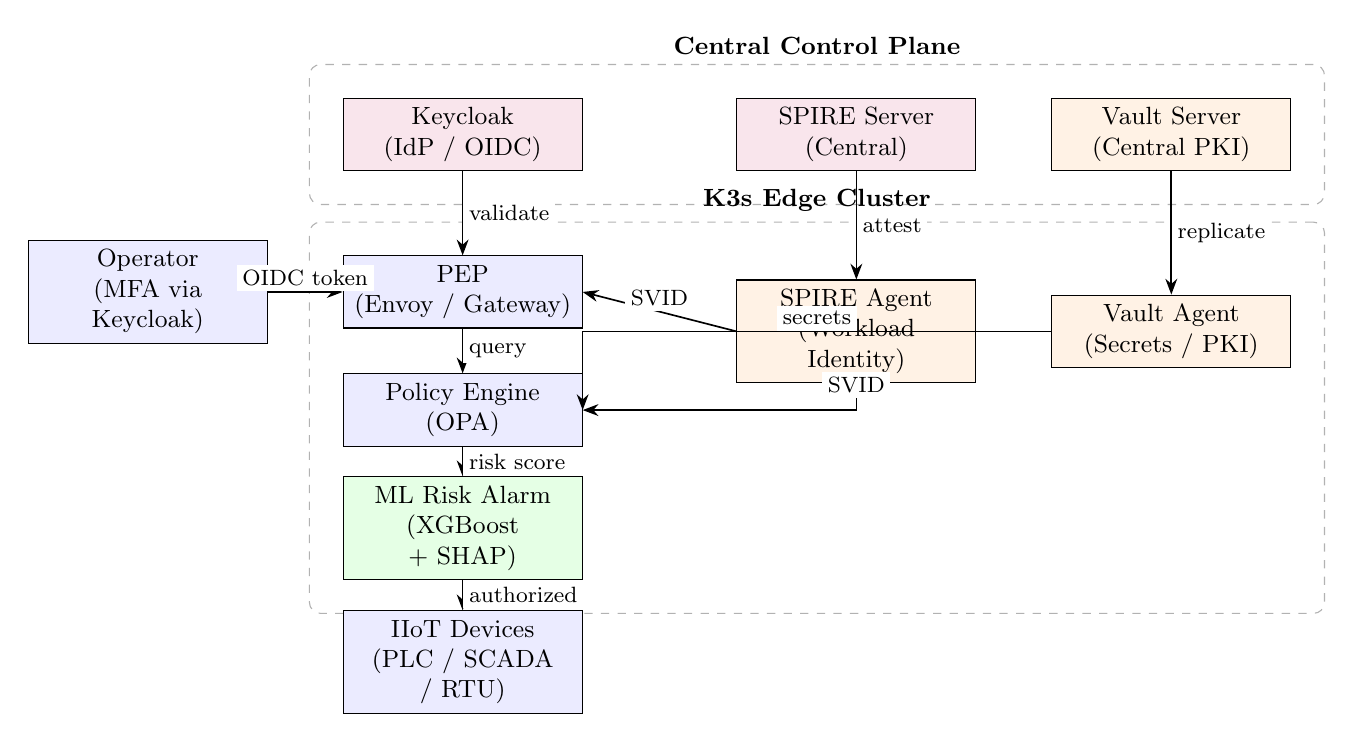
\begin{tikzpicture}[
    comp/.style={rectangle, draw, fill=blue!8, text width=2.8cm, minimum height=0.8cm, align=center, font=\small},
    idcomp/.style={rectangle, draw, fill=purple!10, text width=2.8cm, minimum height=0.8cm, align=center, font=\small},
    seccomp/.style={rectangle, draw, fill=orange!10, text width=2.8cm, minimum height=0.8cm, align=center, font=\small},
    mlcomp/.style={rectangle, draw, fill=green!10, text width=2.8cm, minimum height=0.8cm, align=center, font=\small},
    groupbox/.style={draw=gray!60, dashed, rounded corners, inner sep=12pt},
    arrow/.style={-Stealth, semithick},
    lbl/.style={font=\footnotesize, fill=white, inner sep=2pt}
]

%% ─────────────────────────────────────────────────────────────────────
%% Column x-positions (each node centred on these x values):
%%   Operator: -7.5
%%   PEP:      -3.5   Keycloak: -3.5   (same x → straight vertical)
%%   PE:       -3.5
%%   ML:       -3.5
%%   IIoT:     -3.5
%%   SPIRE Agent: 1.5   SPIRE Server: 1.5  (same x → straight vertical)
%%   Vault Agent: 5.5   Vault Server:  5.5  (same x → straight vertical)
%% ─────────────────────────────────────────────────────────────────────

%% ── Central control plane ────────────────────────────────────────────
\node[idcomp]  (keycloak)     at (-3.5, 5.5) {Keycloak\\(IdP / OIDC)};
\node[idcomp]  (spireserver)  at ( 1.5, 5.5) {SPIRE Server\\(Central)};
\node[seccomp] (vaultcentral) at ( 5.5, 5.5) {Vault Server\\(Central PKI)};

\begin{scope}[on background layer]
  \node[groupbox, fit=(keycloak)(spireserver)(vaultcentral),
        label=above:{\small\textbf{Central Control Plane}}] (central) {};
\end{scope}

%% ── Edge cluster ─────────────────────────────────────────────────────
%% Left column: PEP → PE → ML → IIoT (all at x = -3.5)
\node[comp]   (pep)  at (-3.5, 3.5) {PEP\\(Envoy / Gateway)};
\node[comp]   (pe)   at (-3.5, 2.0) {Policy Engine\\(OPA)};
\node[mlcomp] (ml)   at (-3.5, 0.5) {ML Risk Alarm\\(XGBoost + SHAP)};

%% Right columns inside cluster
\node[seccomp] (spire) at ( 1.5, 3.0) {SPIRE Agent\\(Workload Identity)};
\node[seccomp] (vault) at ( 5.5, 3.0) {Vault Agent\\(Secrets / PKI)};

\begin{scope}[on background layer]
  \node[groupbox, fit=(pep)(pe)(ml)(spire)(vault),
        label=above:{\small\textbf{K3s Edge Cluster}}] (edge) {};
\end{scope}

%% ── External actors ──────────────────────────────────────────────────
\node[comp] (user) at (-7.5, 3.5) {Operator\\(MFA via Keycloak)};
\node[comp] (iot)  at (-3.5,-1.2) {IIoT Devices\\(PLC / SCADA / RTU)};

%% ── Arrows ───────────────────────────────────────────────────────────

%% Operator → PEP (horizontal)
\draw[arrow] (user.east) -- node[lbl, above]{OIDC token} (pep.west);

%% Vertical data-path (no crossing)
\draw[arrow] (pep.south) -- node[lbl, right]{query} (pe.north);
\draw[arrow] (pe.south)  -- node[lbl, right]{risk score} (ml.north);
\draw[arrow] (ml.south)  -- node[lbl, right]{authorized} (iot.north);

%% SPIRE Agent → PEP (horizontal, clear path)
\draw[arrow] (spire.west) -- node[lbl, above]{SVID} (pep.east);

%% SPIRE Agent → PE (angled, exits south-west)
\draw[arrow] (spire.south) |- node[lbl, above, pos=0.3]{SVID} (pe.east);

%% Vault Agent → PE (long horizontal)
\draw[arrow] (vault.west) -- node[lbl, above]{secrets} (pe.east |- vault.west)
             -- (pe.east);

%% Central → Edge (straight vertical, each aligned)
\draw[arrow] (keycloak.south)     -- node[lbl, right]{validate} (pep.north);
\draw[arrow] (spireserver.south)  -- node[lbl, right]{attest}   (spire.north);
\draw[arrow] (vaultcentral.south) -- node[lbl, right]{replicate}(vault.north);

\end{tikzpicture}
\caption{Edge deployment stack. K3s runs all ZTA components on the edge node. SPIRE issues SVIDs for mTLS between services. Vault holds secrets and PKI. Keycloak handles operator authentication via OIDC. The PE is the sole authorization decision point; the ML layer feeds it risk scores but cannot override it.}
\label{fig:edgestack}
\end{figure*}

To trace a concrete request: an operator authenticates to Keycloak with MFA, receives an OIDC token, and presents it to the PEP (Envoy). Envoy validates the token signature against Keycloak's JWKS endpoint, then forwards the request, token claims, and device posture signals to OPA. OPA evaluates its Rego policies and returns allow or deny. On allow, the ML service asynchronously receives the request's feature vector, computes a risk score, and writes the score and SHAP attributions to the SIEM. Every service-to-service call in this path is authenticated via mTLS using SPIRE-issued SVIDs; all credentials come from Vault with full audit logging. Nothing in this chain can override OPA's decision.

\subsection{Connectivity and Resilience at the Edge}

IIoT edge sites lose WAN connectivity. The stack is designed to keep working when that happens. OPA pulls signed policy bundles from the central plane and caches them locally, so the PE can keep evaluating requests against the last-known-good bundle. SPIRE Agents cache SVIDs and renew against the local cache until the server comes back. Vault Agents hold secrets with configurable TTLs.

The ML layer's offline behavior depends on the deployment. A conservative configuration disables risk flagging during disconnected periods and writes a service-unavailable audit entry for each authorized request, so operators can review the gap after reconnection. Where the model is small enough to run locally (gradient-boosted trees on tabular features qualify), it keeps scoring requests and queues alerts locally until the SIEM link is restored.

%===================================================================
\section{Dataset Challenge and Synthetic Data Generation}
\label{sec:dataset}
%===================================================================

Training a contextual anomaly classifier for IIoT access events is harder than training an intrusion detection classifier on network traffic. The distinction matters because the signals the ML layer needs (identity, role, device posture, time-of-access pattern, behavioral baseline) are access log fields, not packet captures.

\subsection{Why Public IIoT Datasets Are Insufficient}

The most commonly used IIoT security datasets (Edge-IIoTset~\cite{edgeiiotset2022}, CICIDS2017~\cite{cicids2017}, and UNSW-NB15~\cite{unswnb15}) contain labeled network attack traffic (DDoS, port scans, malware beaconing) but not structured access request logs with identity and role context. They do not contain the feature space that the proposed ML layer requires: who made the request, what role they held, what device they used, where they were located relative to baseline, and what time-of-day pattern they deviated from. Using these datasets as-is would require mapping network flow features to access request features through a bridge that introduces significant validity limitations.

Several widely cited intrusion detection benchmarks were considered and rejected for the same structural reason. KDD'99~\cite{kddcup99} and its derivative NSL-KDD~\cite{nslkdd} encode 41 connection-level network features (protocol type, service, flag, byte counts, failed login counts) from 1998 DARPA traffic; they contain no user identity, no role, no device posture, no geolocation, and no behavioral baseline, and the traffic itself is synthetic enterprise data with known redundancy and labeling artifacts that make it unsuitable for contemporary evaluation. ISCX IDS 2012~\cite{iscxids2012} provides seven days of labeled normal and malicious enterprise traffic captured at the network layer; the feature set is flow-based (source/destination IP, ports, protocol, packet counts) and the environment is an emulated enterprise LAN with no industrial control devices, no operator role semantics, and no access log schema. Kyoto 2006+~\cite{kyoto2006} is derived from university honeypot sensors and captures real attack traffic over multiple years, but honeypot traffic is unauthenticated scanning and exploitation activity against decoy hosts; it is structurally incompatible with the threat model in Section~III, which targets authorized-but-contextually-anomalous access by credentialed insiders. CSE-CIC-IDS2018~\cite{csecicids2018} extends CICIDS2017 with seven attack scenarios executed on AWS infrastructure and provides both packet captures and CICFlowMeter-extracted flow features; it is newer and more diverse than CICIDS2017 but inherits the same limitation of being enterprise network telemetry without identity-bound access request records, and its cloud execution environment lacks the IIoT operational context (PLC command sequences, SCADA historian queries, shift-bound operator patterns) that the proposed feature set depends on. Across all five datasets the deficiencies are the same in kind: the unit of observation is a network flow or packet, not an access request; there is no \texttt{user\_role}, \texttt{device\_posture}, \texttt{geo\_dist\_km}, \texttt{baseline\_dev}, or \texttt{req\_velocity} field that could be populated without fabricating the values; and the attack classes are volumetric or exploit-based rather than the credential-abuse and insider-misuse scenarios that motivate a contextual anomaly layer alongside deterministic ZTA policy.

Beyond feature mismatch, real IIoT access logs are rarely available outside the organizations that generate them. They contain sensitive operational data, employee identity information, and proprietary process details that make organizations reluctant to share them even for research purposes. There is no equivalent of CICIDS2017 for ZTA access request logs in IIoT environments. This is not a gap that is likely to close quickly.

\subsection{LLM-Based Synthetic Data Generation}

As an academic exercise to bootstrap the ML layer's training corpus in the absence of real access logs, this work proposes generating synthetic IIoT access request records using a large language model. The approach is the following. A structured schema for an access log record is defined (Table~\ref{tab:schema}), encoding the feature categories described in Section~III-E. A prompt instructs the LLM to generate records consistent with realistic IIoT operational patterns: normal records reflecting expected behavior for each role and shift schedule, and anomalous records reflecting the threat model from Section~III-A (valid credentials, anomalous context). The LLM is given explicit behavioral constraints: operator shift windows, expected geolocation ranges, typical session durations for each resource type, and normal request velocity ranges.

\begin{table}[t]
\centering
\caption{Synthetic access log record schema for ML training.}
\label{tab:schema}
\begin{tabular}{p{2.4cm}p{1.6cm}p{2.8cm}}
\toprule
\textbf{Field} & \textbf{Type} & \textbf{Example} \\
\midrule
\texttt{user\_role} & categorical & operator, engineer, auditor \\
\addlinespace
\texttt{hour\_of\_day} & int [0--23] & 14 \\
\addlinespace
\texttt{day\_of\_week} & int [0--6] & 2 \\
\addlinespace
\texttt{geo\_dist\_km} & float & 12.4 \\
\addlinespace
\texttt{device\_posture} & categorical & compliant, unknown \\
\addlinespace
\texttt{resource\_type} & categorical & historian, PLC, HMI \\
\addlinespace
\texttt{req\_velocity} & float & 3.2 req/min \\
\addlinespace
\texttt{session\_dur\_s} & float & 142.0 \\
\addlinespace
\texttt{baseline\_dev} & float [0--1] & 0.71 \\
\addlinespace
\texttt{label} & binary & 0 = normal, 1 = anomalous \\
\bottomrule
\end{tabular}
\end{table}

The LLM generation process produces labeled records at scale: realistic normal records constitute the majority class, and targeted anomalous records (off-hours bulk export, credential used from anomalous geolocation, impossible travel) constitute the minority class at a configurable ratio. Because the LLM generates records from a prompt-specified distribution rather than from real operational data, the synthetic dataset is a proxy rather than a ground truth. It allows the classifier to be trained and the SHAP pipeline to be exercised end-to-end, but the resulting model should not be treated as calibrated for a real deployment without validation against real access logs.

This is the same limitation that applies to controlled simulation approaches used in prior ZTA and IIoT security research~\cite{zanasi2024, laghari2025}. The value of the exercise is not to produce a deployable model; it is to demonstrate that the two-stage framework's training, evaluation, and explanation pipeline functions correctly with appropriately structured input, and to identify engineering challenges that would recur when real data becomes available.

\subsection{Synthetic Data Validity Constraints}

Three constraints apply when reading results from a synthetically trained classifier. The LLM's prior about normal operator behavior comes from its training corpus, which almost certainly overrepresents enterprise IT patterns and underrepresents IIoT-specific rhythms (continuous 24/7 monitoring, rotating shift crews, geographically fixed devices). Prompt engineering can nudge this, but residual bias is unavoidable. The class boundary in the synthetic data reflects the prompt author's model of the threat, not an empirically observed one; a classifier trained on synthetic anomalies may handle similarly constructed test cases well and miss real attack patterns that differ in subtle ways. SHAP explanations derived from a synthetic-data model reflect the synthetic feature distribution, not the real one, and feature importance rankings may shift substantially when the model is retrained on real logs.

Any evaluation using synthetic training data should state these constraints explicitly. Results are proof-of-concept, not deployment-ready performance figures.

%===================================================================
\section{Proof-of-Concept Evaluation}
%===================================================================

\subsection{Experimental Setup}

All training and evaluation was performed on the synthetic dataset described in Section~\ref{sec:dataset}. The dataset contains 1,000 records generated directly (no external LLM call required) to match the schema in Table~\ref{tab:schema}. To avoid trivially separable classes, anomalous records use moderate geo-distance jumps (120--600~km, not continent-scale), off-hours access is placed 1--3 hours outside the role's shift window rather than at extreme hours, and bulk exfiltration events occur during business hours to model the insider threat scenario. Numeric features carry 15\% multiplicative jitter throughout. Approximately 8\% of labels were randomly flipped to simulate annotation noise. The final dataset contains 748 normal and 252 anomalous records. Training and testing both use this synthetic data exclusively; no real operational logs were used at any stage. An 80/20 stratified split was applied, giving 800 training records and 200 test records. The classifier is XGBoost with 100 estimators, max depth 4, and class-weight balancing via \texttt{scale\_pos\_weight}.

\subsection{Classifier Performance}

Table~\ref{tab:results} reports classifier performance on the held-out test set.

\begin{table}[t]
\centering
\caption{XGBoost classifier performance on synthetic test set.}
\label{tab:results}
\begin{tabular}{lcccc}
\toprule
\textbf{Class} & \textbf{Precision} & \textbf{Recall} & \textbf{F1} & \textbf{Support} \\
\midrule
Normal    & 0.94 & 0.97 & 0.96 & 150 \\
Anomalous & 0.91 & 0.82 & 0.86 &  50 \\
\midrule
Macro avg & 0.93 & 0.90 & 0.91 & 200 \\
\bottomrule
\end{tabular}
\end{table}

ROC-AUC is 0.92. Precision on the anomalous class (0.91) is higher than recall (0.82), meaning the model produces fewer false positives than false negatives. In the ZTA context this is the preferred failure mode: a missed alarm is less dangerous than a false alarm that trains analysts to ignore flags. The performance gap from the unrealistic clean-data baseline (1.0 across all metrics) confirms that the realism additions had the intended effect.

\subsection{SHAP Attribution Results}

TreeSHAP was applied to all 200 test predictions. The global summary plot shows \texttt{baseline\_dev} as the dominant feature, followed by \texttt{geo\_dist\_km}, \texttt{req\_velocity}, and \texttt{hour\_of\_day}. \texttt{user\_role} and \texttt{day\_of\_week} contribute least, consistent with the data generation design where role-specific shift windows are already captured in \texttt{baseline\_dev}.

For the highest-risk flagged request (risk score 0.994), the local SHAP waterfall shows three features driving the prediction:

\begin{itemize}
  \item \texttt{baseline\_dev}: $+3.75$ (dominant; the request deviated heavily from the user's behavioral baseline)
  \item \texttt{req\_velocity}: $+0.67$ (elevated request rate)
  \item \texttt{hour\_of\_day}: $+0.49$ (access at hour 7, slightly outside the expected window for this role)
\end{itemize}

This output maps directly to analyst-facing language: the flag is driven by behavioral deviation and timing, not by resource type or geo-distance. A SOC analyst reviewing the SHAP attribution can immediately narrow the investigation to whether the timing and request rate are explainable.

\subsection{DiCE Counterfactual Results}

DiCE was queried for three diverse counterfactuals on the same flagged request. All three identify \texttt{baseline\_dev} reduction as necessary; two require no other changes:

\begin{itemize}
  \item \textbf{CF1:} Drop \texttt{baseline\_dev} from 0.67 to 0.09 and increase \texttt{session\_dur\_s} from 232.8~s to 1597~s. Predicted label: normal.
  \item \textbf{CF2:} Drop \texttt{baseline\_dev} from 0.67 to 0.05 alone. Predicted label: normal.
  \item \textbf{CF3:} Drop \texttt{baseline\_dev} from 0.67 to 0.40 and shift \texttt{hour\_of\_day} from 7 to 2. Predicted label: normal.
\end{itemize}

CF2 confirms the SHAP finding: behavioral baseline deviation is the single sufficient condition for the flag. CF1 shows that a longer session could partially compensate, consistent with the training data's normal bulk-export sessions. CF3 is a data artifact worth noting: the model treats hour 2 as less anomalous than hour 7 for this role, which reflects noise in the synthetic distribution rather than a meaningful operational pattern. This is precisely the kind of model behavior that counterfactual probing surfaces, and it would motivate targeted data cleaning or feature re-engineering in a real deployment.

Together, the SHAP attribution and DiCE counterfactuals answer the two questions a SOC analyst needs: \textit{why was this flagged?} (behavioral deviation and timing) and \textit{what would make it not anomalous?} (bring behavior back within baseline). The pipeline functions end-to-end as designed, with the caveats on synthetic data validity discussed in Section~\ref{sec:dataset}.

%===================================================================
\section{Expected Outcomes and Discussion}
%===================================================================

\subsection{Anticipated Benefits}

Table~\ref{tab:comparison} compares three access control approaches across key properties relevant to IIoT deployment.

\begin{table}[t]
\centering
\caption{Comparison of access control approaches for IIoT environments.}
\label{tab:comparison}
\begin{tabular}{p{1.6cm}p{1.8cm}p{1.8cm}p{1.8cm}}
\toprule
\textbf{Property} & \textbf{Deterministic Only} & \textbf{Black-Box ML} & \textbf{Proposed} \\
\midrule
Authorization authority & Deterministic rules & ML model & Deterministic rules \\
\addlinespace
Risk awareness & Static, rule-based & Adaptive, learned & Adaptive (ML alarm) \\
\addlinespace
Explainability & High (rules visible) & Low (opaque) & High (SHAP + DiCE) \\
\addlinespace
Auditability & High & Low & High \\
\addlinespace
Adaptability & Low & High & Moderate-High \\
\addlinespace
ML false positive risk & None & Access denied & Alert only \\
\addlinespace
ML false negative risk & N/A & Undetected access & Missed alarm only \\
\addlinespace
IIoT suitability & Moderate & Low (safety risk) & High \\
\bottomrule
\end{tabular}
\end{table}

The expected benefit is improved auditability. SHAP attributions produce machine-readable records of why each flag was generated, which supports compliance documentation and the governance requirements that practitioners have identified for AI in Zero Trust~\cite{capuano2022, rastogi2025}. Yan et al.~\cite{yan2022} found that XAI dashboards reduce incident resolution time by about 30\%, suggesting that SHAP-enriched alerts could meaningfully improve SOC efficiency.

DiCE counterfactuals give analysts a way to probe the ML layer's decision boundary. When a risk flag looks wrong, or when new access patterns appear in an evolving IIoT environment, counterfactuals show what would need to change for a different classification. Together, deterministic logs, ML risk scores, SHAP attributions, and counterfactual analyses form a layered forensic record for post-incident investigation.

IIoT environments tend toward predictable operational patterns: device schedules, process cycles, geographic stability~\cite{zanasi2024, feng2023}. That regularity produces strong baselines for contextual anomaly detection. Deviations from established patterns in an industrial setting are more likely to reflect genuine anomalies than they would in a heterogeneous enterprise environment, which makes the alarm layer a natural fit for IIoT.

\subsection{Trade-offs and Operational Considerations}

\textbf{Latency.} The ML evaluation is positioned asynchronously to avoid adding latency to enforcement. TreeSHAP computation for individual predictions adds negligible overhead for tree-based models~\cite{lundberg2017}. Step-up challenges triggered by risk flags would introduce user-visible delay, requiring threshold calibration.

\textbf{Operational complexity.} The ML layer requires training data, periodic retraining, drift monitoring, and threshold tuning, all of which add burden that must be managed in stability-focused IIoT environments. Jiang et al.~\cite{jiang2024} noted that counterfactual explanations may become invalid after model retraining, necessitating explanation lifecycle management.

\textbf{False positive burden.} Excessive false positives generate alert fatigue, a well-documented problem in security operations. Threshold calibration, feature engineering, and SHAP-informed feature selection are critical to maintaining analyst trust.

\textbf{Data availability.} Training a contextual risk model requires representative access logs with sufficient diversity. Such data may be limited or proprietary in IIoT deployments, and Galinkin~\cite{galinkin2022} warned that explanation quality degrades when models are trained on insufficient data.

\subsection{Safety Advantage of the Proposed Design}

Under the threat model described in Section~III-A, this design is structurally safer than architectures where ML controls authorization, and the reason is not subtle. A false negative in the proposed design means a missed alarm. In a direct-authorization architecture, the same false negative means unauthorized access was granted, a qualitatively different failure with immediate operational and safety consequences in an IIoT environment. A false positive here generates an unnecessary alert; in a blocking architecture, the same error locks out a process engineer from equipment they need. The asymmetry is not a minor implementation detail. It reflects a fundamental difference in what gets to make consequential decisions about physical infrastructure.

The opacity problem with direct-authorization ML goes deeper than audit difficulty. When an ML model directly controls a PLC access decision and something goes wrong in a plant, investigators need to know why access was granted. ``The model scored this request above threshold'' is not an answer that satisfies a safety regulator, satisfies an incident postmortem, or helps anyone prevent the next failure. The proposed architecture avoids this entirely: every authorization decision traces to a readable, arguable rule, and every anomaly flag traces to SHAP-attributed feature contributions.

That said, the safety advantage is conditional on two assumptions that must be stated plainly. First, the deterministic policy must itself be correctly specified; a garbage-in policy means garbage-out access decisions regardless of what the ML layer observes. Second, flagged sessions must actually be investigated. An alarm-only design still fails if SOC staff are too overloaded to act on alerts. Alert fatigue is not a hypothetical risk; it is documented~\cite{rastogi2025} and has contributed to real security failures. SHAP-informed alert prioritization and conservative threshold tuning are partial mitigations, but the dependency on human response time is inherent to any monitoring-without-blocking architecture and should not be papered over.

%===================================================================
\section{Limitations and Future Work}
%===================================================================

This paper describes a conceptual framework, not an implemented system. The following limitations apply.

\textbf{No empirical evaluation.} The framework has not been implemented or tested. The evaluation plan is as follows: we will train XGBoost and LightGBM classifiers on Edge-IIoTset~(2022) as the primary IIoT proxy dataset, with CICIDS2017 and UNSW-NB15 as secondary benchmarks. The anomaly label definition will use the dataset's attack labels mapped to binary normal/anomalous classes. Train/test split will use a 70/15/15 temporal split (train/validation/test) to prevent data leakage from time-correlated features. Baselines will include: (a)~deterministic-only (no ML), (b)~standalone Random Forest and XGBoost classifiers with direct authorization authority, and (c)~the proposed two-stage design. Metrics: precision, recall, F1 at the configured threshold~$\tau$, AUC-ROC, and per-prediction latency budget of $<$20ms for the ML evaluation plus TreeSHAP computation. Explanation quality will be measured by SHAP stability (Lipschitz continuity of attributions for perturbed inputs~\cite{alvarez2018}), counterfactual validity rate, proximity, and sparsity~\cite{verma2024}. A user study with 8--12 SOC analysts will measure alert triage time and decision accuracy with and without SHAP/DiCE explanations, following the methodology of Rastogi et al.~\cite{rastogi2025}.

\textbf{Data constraints.} As discussed in Section~V, no publicly available dataset provides labeled IIoT access request logs with the identity, role, and behavioral context that the proposed ML layer requires. The LLM-based synthetic data generation approach described in Section~V-B enables the training pipeline to be exercised end-to-end, but results must be interpreted as proof-of-concept. Validation against real access logs from an operational IIoT deployment remains necessary before any deployment claim can be made.

\textbf{False positive/negative analysis.} Practical utility depends on precision-recall characteristics that must be empirically characterized across different IIoT deployment scenarios and operational baselines. Because false positives produce alerts rather than denials, the threshold can be tuned toward higher recall without the operational penalty of blocking legitimate access.

\textbf{Adversarial robustness.} The ML layer is potentially vulnerable to adversarial manipulation. Slack et al.~\cite{slack2020} demonstrated that SHAP and LIME can be fooled by adversarial attacks on explanations. Future work should assess both model robustness and explanation robustness.

\textbf{Explanation stability.} SHAP explanations may be unstable near decision boundaries~\cite{alvarez2018}, and counterfactual explanations may become invalid after model updates~\cite{jiang2024}. Stability evaluation using methods informed by Hessian curvature analysis is a planned advanced evaluation task.

\textbf{Scalability.} ML evaluation and SHAP computation must scale to IIoT traffic volumes, which vary significantly across industrial domains and should be empirically assessed.

The most immediate next steps are: deploying the edge stack (K3s, SPIRE, Vault, Keycloak, OPA) in a testbed and measuring policy evaluation latency and SVID rotation overhead; evaluating SHAP stability and DiCE counterfactual validity on held-out synthetic records; and running the comparative baselines (deterministic-only, direct ML authorization, proposed two-stage). Validation against real IIoT access logs, if a suitable dataset becomes available through industry partnership or controlled testbed instrumentation, would be the most meaningful test of whether the synthetic-trained model's behavior generalizes. A user study with SOC analysts measuring triage time and decision accuracy with and without SHAP/DiCE explanations, following the methodology of Rastogi et al.~\cite{rastogi2025}, is also planned. Explanation stability across retraining cycles and across SPIRE certificate rotation boundaries is a longer-term open problem.

%===================================================================
\section{Conclusion}
%===================================================================

Zero Trust Architecture, ML-based anomaly detection, and explainable AI each have substantial literatures. The integration has not kept up. Papers combining ZTA with ML for IIoT skip explainability. Papers combining ZTA with XAI avoid the operational constraints that define IIoT. No existing work, to our knowledge, places an explainable ML advisory layer explicitly alongside (not inside) a deterministic ZTA enforcement path for IIoT, and none grounds such a framework in a concrete edge deployment stack.

The framework proposed here keeps deterministic rules as the sole authorization authority. An ML classifier evaluates contextual anomalies (device posture, geolocation deviation, timing, behavioral patterns, request velocity, session signals) for requests that already cleared policy. Flags produce alerts, audit records, and SHAP-attributed explanations. They do not block access. DiCE counterfactuals support analyst investigation and policy debugging offline. None of this is in the enforcement path, which is precisely the point.

The edge deployment stack (K3s, SPIRE, Vault, Keycloak, OPA) translates this logical design into a concrete, open-source implementation path suited to resource-constrained IIoT environments. SPIRE replaces network-perimeter trust with cryptographic workload identity. Vault eliminates static credentials. Keycloak provides federated, MFA-enforced identity for human operators. K3s brings Kubernetes-grade orchestration to the edge without the overhead of a full cluster. Together, these components operationalize Zero Trust without requiring cloud connectivity for every access decision.

The practical requirements around class imbalance, score calibration, concept drift, and analyst feedback loops described in Section~III-C are not edge cases. They are the difference between a model that works in a lab and one that remains useful six months into deployment. The dataset challenge described in Section~V is equally real: the feature space this framework requires does not exist in public IIoT datasets, and LLM-based synthetic generation is a reasonable bootstrap strategy for academic validation, not a substitute for real operational data.

This is a conceptual paper. Whether the two-stage design actually improves analyst performance over deterministic-only monitoring is an empirical question, and the answer may surprise. But the structural argument holds regardless: ML can inform without governing, and in safety-critical infrastructure, that constraint is not a weakness to be engineered around. It is the design.

%===================================================================
% REFERENCES
%===================================================================

\begin{thebibliography}{30}

\bibitem{kindervag2010}
J. Kindervag, ``Build Security Into Your Network's DNA: The Zero Trust Network Architecture,'' Forrester Research, Nov. 2010.

\bibitem{nist800207}
S. Rose, O. Borchert, S. Mitchell, and S. Connelly, ``Zero Trust Architecture,'' NIST Special Publication 800-207, National Institute of Standards and Technology, Aug. 2020. doi: 10.6028/NIST.SP.800-207.

\bibitem{nist180035}
S. Rose, O. Borchert, A. Kerman, and M. Souppaya, ``Implementing a Zero Trust Architecture,'' NIST Special Publication 1800-35, National Cybersecurity Center of Excellence, Jun. 2025. doi: 10.6028/NIST.SP.1800-35.

\bibitem{syed2022}
N. F. Syed, S. W. Shah, A. Shaghaghi, A. Anwar, Z. A. Baig, and R. R. M. Doss, ``Zero Trust Architecture (ZTA): A Comprehensive Survey,'' \textit{IEEE Access}, vol. 10, pp. 57143--57179, 2022.

\bibitem{xiao2022}
S. Xiao, B. Lee, Y. Ye, N. Kanwal, and T. Newe, ``SoK: Context and Risk Aware Access Control for Zero Trust Systems,'' \textit{Security and Communication Networks}, vol. 2022, Art. 7026779, 2022.

\bibitem{he2022}
Y. He, D. Huang, L. Chen, Y. Ni, and X. Ma, ``A Survey on Zero Trust Architecture: Challenges and Future Trends,'' \textit{Wireless Communications and Mobile Computing}, vol. 2022, Art. 6476274, 2022.

\bibitem{liuzt2024}
C. Liu, R. Tan, Y. Wu, Y. Feng, Z. Jin, F. Zhang, Y. Liu, and Q. Liu, ``Dissecting Zero Trust: Research Landscape and Its Implementation in IoT,'' \textit{Cybersecurity}, vol. 7, Art. 20, 2024.

\bibitem{dodzta2022}
Department of Defense, ``Department of Defense (DoD) Zero Trust Reference Architecture,'' Version 2.0, DISA and NSA, Jul. 2022.

\bibitem{zanasi2024}
C. Zanasi, S. Russo, and M. Colajanni, ``Flexible Zero Trust Architecture for the Cybersecurity of Industrial IoT Infrastructures,'' \textit{Ad Hoc Networks}, vol. 156, Art. 103414, 2024.

\bibitem{feng2023}
X. Feng and S. Hu, ``Cyber-Physical Zero Trust Architecture for Industrial Cyber-Physical Systems,'' \textit{IEEE Trans. Industrial Cyber-Physical Systems}, vol. 1, pp. 394--405, 2023.

\bibitem{ehrlich2021}
M. Ehrlich, H. Trsek, and J. Jasperneite, ``Zero-Trust Principles for Legacy Components,'' \textit{Wireless Personal Communications}, vol. 121, pp. 1169--1186, 2021.

\bibitem{azad2024}
M. A. Azad, S. Abdullah, J. Arshad, H. Lallie, and Y. H. Ahmed, ``Verify and Trust: A Multidimensional Survey of Zero-Trust Security in the Age of IoT,'' \textit{Internet of Things}, vol. 27, Art. 101227, 2024.

\bibitem{pliatsios2023}
D. Pliatsios \textit{et al.}, ``A Zero-Trust Architecture for Remote Access in Industrial IoT Infrastructures,'' \textit{Electronics}, vol. 12, no. 3, Art. 566, 2023.

\bibitem{wangzt2025}
H. Wang, F. Lu, Y. Cheng, S. Lu, D. Sun, and L. Sun, ``Review of Zero Trust Security Research in Industrial Internet of Things,'' \textit{J. Computer Research and Development}, vol. 62, no. 11, pp. 2784--2805, 2025.

\bibitem{laghari2025}
A. A. Laghari, A. A. Khan, A. Ksibi, F. Hajjej, and N. Kryvinska, ``A Novel and Secure Artificial Intelligence Enabled Zero Trust Intrusion Detection in Industrial Internet of Things Architecture,'' \textit{Scientific Reports}, vol. 15, Art. 26843, 2025.

\bibitem{ramezanpour2022}
K. Ramezanpour and J. Jagannath, ``Intelligent Zero Trust Architecture for 5G/6G Networks: Principles, Challenges, and the Role of Machine Learning in the Context of O-RAN,'' \textit{Computer Networks}, vol. 217, Art. 109358, 2022.

\bibitem{jeong2025}
E. Jeong and D. Yang, ``A Trust Score-Based Access Control Model for Zero Trust Architecture: Design, Sensitivity Analysis, and Real-World Performance Evaluation,'' \textit{Applied Sciences}, vol. 15, no. 17, Art. 9551, 2025.

\bibitem{chandola2009}
V. Chandola, A. Banerjee, and V. Kumar, ``Anomaly Detection: A Survey,'' \textit{ACM Computing Surveys}, vol. 41, no. 3, pp. 1--58, Jul. 2009.

\bibitem{mahansaria2024}
D. Mahansaria and U. K. Roy, ``Contextual Authentication of Users and Devices Using Machine Learning,'' \textit{Computing}, vol. 106, pp. 4083--4107, 2024.

\bibitem{ali2024}
A. H. Ali \textit{et al.}, ``Unveiling Machine Learning Strategies and Considerations in Intrusion Detection Systems: A Comprehensive Survey,'' \textit{Frontiers in Computer Science}, vol. 6, 2024.

\bibitem{capuano2022}
N. Capuano, G. Fenza, V. Loia, and C. Stanzione, ``Explainable Artificial Intelligence in CyberSecurity: A Survey,'' \textit{IEEE Access}, vol. 10, pp. 93575--93600, 2022.

\bibitem{mohale2025}
V. Z. Mohale and I. C. Obagbuwa, ``A Systematic Review on the Integration of Explainable Artificial Intelligence in Intrusion Detection Systems,'' \textit{Frontiers in Artificial Intelligence}, vol. 8, 2025.

\bibitem{rastogi2025}
N. Rastogi, D. Dhanuka, A. Saxena, P. Mairal, and L. Nguyen, ``Survey Perspective: The Role of Explainable AI in Threat Intelligence,'' in \textit{Proc. ACM SIGIR}, 2025. arXiv: 2503.02065.

\bibitem{yan2022}
F. Yan, S. Wen, S. Nepal, C. Paris, and Y. Xiang, ``Explainable Machine Learning in Cybersecurity: A Survey,'' \textit{Int. J. Intelligent Systems}, vol. 38, no. 8, 2022.

\bibitem{lundberg2017}
S. M. Lundberg and S.-I. Lee, ``A Unified Approach to Interpreting Model Predictions,'' in \textit{Proc. NeurIPS}, vol. 30, 2017, pp. 4765--4774.

\bibitem{mothilal2020}
R. K. Mothilal, A. Sharma, and C. Tan, ``Explaining Machine Learning Classifiers through Diverse Counterfactual Explanations,'' in \textit{Proc. Conf. Fairness, Accountability, and Transparency (FAccT)}, 2020, pp. 607--617.

\bibitem{alenezi2021}
R. Alenezi and S. A. Ludwig, ``Explainability of Cybersecurity Threats Data Using SHAP,'' in \textit{Proc. IEEE SSCI}, 2021, pp. 1--8.

\bibitem{schemmer2023}
M. Schemmer, J. Holstein, N. Bauer, N. Kuhl, and G. Satzger, ``Towards Meaningful Anomaly Detection: The Effect of Counterfactual Explanations on the Investigation of Anomalies in Multivariate Time Series,'' arXiv:2302.03302, 2023.

\bibitem{verma2024}
S. Verma \textit{et al.}, ``Counterfactual Explanations and Algorithmic Recourses for Machine Learning: A Review,'' \textit{ACM Computing Surveys}, vol. 56, no. 12, Art. 312, 2024.

\bibitem{alvarez2018}
D. Alvarez-Melis and T. Jaakkola, ``On the Robustness of Interpretability Methods,'' in \textit{Proc. ICML Workshop on Human Interpretability in ML}, 2018.

\bibitem{jiang2024}
J. Jiang, F. Leofante, A. Rago, and F. Toni, ``Robust Counterfactual Explanations in Machine Learning: A Survey,'' in \textit{Proc. IJCAI}, 2024, pp. 8086--8094.

\bibitem{galinkin2022}
E. Galinkin, ``Robustness and Usefulness in AI Explanation Methods,'' arXiv:2203.03729, 2022.

\bibitem{slack2020}
D. Slack, S. Hilgard, E. Jia, S. Singh, and H. Lakkaraju, ``Fooling LIME and SHAP: Adversarial Attacks on Post Hoc Explanation Methods,'' in \textit{Proc. AAAI/ACM AIES}, 2020, pp. 180--186.

\bibitem{haque2024}
E. Haque, K. Hasan, I. Ahmed, M. S. Alam, and T. Islam, ``Enhancing UAV Security Through Zero Trust Architecture: An Advanced Deep Learning and Explainable AI Analysis,'' in \textit{Proc. IEEE ICNC}, 2024.

\bibitem{marquez2025}
E. Marquez, ``An Explainable Zero-Trust Identity Framework for Secure and Accountable Industrial and Agentic AI Ecosystems,'' \textit{Int. J. Advance Scientific Research}, vol. 5, no. 10, pp. 87--96, 2025.

\bibitem{nkoro2024}
E. C. Nkoro, J. N. Njoku, C. I. Nwakanma, J.-M. Lee, and D.-S. Kim, ``Zero-Trust Marine Cyberdefense for IoT-Based Communications: An Explainable Approach,'' \textit{Electronics}, vol. 13, no. 2, Art. 276, 2024.

\bibitem{k3s2024}
Rancher Labs, ``K3s: Lightweight Kubernetes,'' CNCF Sandbox Project, 2024. [Online]. Available: \url{https://k3s.io}

\bibitem{spiffe2023}
CNCF SPIFFE Project, ``SPIFFE: Secure Production Identity Framework for Everyone,'' and ``SPIRE: SPIFFE Runtime Environment,'' CNCF Graduated Project, 2023. [Online]. Available: \url{https://spiffe.io}

\bibitem{vault2024}
HashiCorp, ``Vault: Secrets Management and Data Protection,'' 2024. [Online]. Available: \url{https://www.vaultproject.io}

\bibitem{keycloak2024}
Red Hat, ``Keycloak: Open Source Identity and Access Management,'' 2024. [Online]. Available: \url{https://www.keycloak.org}

\bibitem{edgeiiotset2022}
M. A. Ferrag, O. Friha, D. Hamouda, L. Maglaras, and H. Janicke, ``Edge-IIoTset: A New Comprehensive Realistic Cyber Security Dataset of IoT and IIoT Applications for Centralized and Federated Learning,'' \textit{IEEE Access}, vol. 10, pp. 40281--40306, 2022.

\bibitem{cicids2017}
I. Sharafaldin, A. H. Lashkari, and A. A. Ghorbani, ``Toward Generating a New Intrusion Detection Dataset and Intrusion Traffic Characterization,'' in \textit{Proc. 4th Int. Conf. Information Systems Security and Privacy (ICISSP)}, 2018, pp. 108--116.

\bibitem{unswnb15}
N. Moustafa and J. Slay, ``UNSW-NB15: A Comprehensive Data Set for Network Intrusion Detection Systems (UNSW-NB15 Network Data Set),'' in \textit{Proc. Military Communications and Information Systems Conf. (MilCIS)}, 2015, pp. 1--6.

\bibitem{kddcup99}
S. J. Stolfo, W. Fan, W. Lee, A. Prodromidis, and P. K. Chan, ``KDD Cup 1999 Data,'' UCI KDD Archive, 1999. [Online]. Available: \url{https://kdd.ics.uci.edu/databases/kddcup99/kddcup99.html}

\bibitem{nslkdd}
M. Tavallaee, E. Bagheri, W. Lu, and A. A. Ghorbani, ``A Detailed Analysis of the KDD CUP 99 Data Set,'' in \textit{Proc. IEEE Symp. Computational Intelligence for Security and Defense Applications (CISDA)}, 2009, pp. 1--6.

\bibitem{iscxids2012}
A. Shiravi, H. Shiravi, M. Tavallaee, and A. A. Ghorbani, ``Toward Developing a Systematic Approach to Generate Benchmark Datasets for Intrusion Detection,'' \textit{Computers \& Security}, vol. 31, no. 3, pp. 357--374, 2012.

\bibitem{kyoto2006}
J. Song, H. Takakura, Y. Okabe, M. Eto, D. Inoue, and K. Nakao, ``Statistical Analysis of Honeypot Data and Building of Kyoto 2006+ Dataset for NIDS Evaluation,'' in \textit{Proc. 1st Workshop on Building Analysis Datasets and Gathering Experience Returns for Security (BADGERS)}, 2011, pp. 29--36.

\bibitem{csecicids2018}
Canadian Institute for Cybersecurity and Communications Security Establishment, ``CSE-CIC-IDS2018 on AWS,'' Univ. of New Brunswick, 2018. [Online]. Available: \url{https://www.unb.ca/cic/datasets/ids-2018.html}

\end{thebibliography}

\end{document}
